%article using font-size 12 and A4-size
\documentclass[a4paper,12pt]{article}

%use danish hyphenation and titles
%handle utf8-characters
\usepackage[danish]{babel}
\usepackage[utf8]{inputenc}
\usepackage[T1]{fontenc}

%for images
\usepackage[pdftex]{graphicx}

%allow nested figures
\usepackage{subfigure}

%control line spacing
\usepackage{setspace}
%\singlespacing
\onehalfspacing
%\doublespacing

%set margins
%\usepackage[margin=0.75in]{geometry}

%allows margin-notes
%good for work in progress papers
%\usepackage{marginnote}

%allows pretty quoting using ``'' or `'
\usepackage{upquote}

%two definitions of the color grey
\usepackage{color}
\definecolor{listinggray}{gray}{0.9}
%\definecolor{lbcolor}{rgb}{0.9,0.9,0.9}

%allows pretty source code
\usepackage{listings}
\lstset{
	language=,
	literate=
		{æ}{{\ae}}1
		{‚àö‚àè}{{\o}}1
		{å}{{\aa}}1
		{‚àö√ú}{{\AE}}1
		{√ò}{{\O}}1
		{√Ö}{{\AA}}1,
	backgroundcolor=\color{listinggray},
	tabsize=3,
	rulecolor=,
	basicstyle=\scriptsize,
	upquote=true,
	aboveskip={1.5\baselineskip},
	columns=fixed,
	showstringspaces=false,
	extendedchars=true,
	breaklines=true,
	prebreak =\raisebox{0ex}[0ex][0ex]{\ensuremath{\hookleftarrow}},
	frame=single,
	showtabs=false,
	showspaces=false,
	showstringspaces=false,
	identifierstyle=\ttfamily,
	keywordstyle=\color[rgb]{0,0,1},
	commentstyle=\color[rgb]{0.133,0.545,0.133},
	stringstyle=\color[rgb]{0.627,0.126,0.941},
}
%captions on listings
\usepackage[center,font=small,labelfont=bf,textfont=it]{caption}

%allows fancy enumeration
\usepackage{enumerate}

%allows use of the BibTex for the bibliography
\usepackage[numbers]{natbib}

%make references and URLs in the pdf to clickable links
\usepackage{hyperref}

%proper header formatting
\usepackage{fancyhdr}
\pagestyle{fancy}
\lhead[]{} %clear standard settings
\chead[]{} %clear standard settings
\rhead[]{\rightmark} %current section
\lfoot[]{} %clear standard settings
\cfoot[]{\thepage} %current page number 
\rfoot[]{} %clear standard settings

%define paper title, author and date
%if date is empty, defaults to current date
\title{Kontekstuel analyse}
\author{Yaser Hashimi og Julie Engholm}
\date{Oktober 9th - 2013}

\begin{document}
\maketitle %insert the defined title
\newpage
\section*{Resume}
\newpage
\tableofcontents %generate table of content
\newpage

\clearpage %clears float-buffer - inserting those missing - and starts new page

\section{PACT analyse}
\subsection{People}
Disse brugere vil man kunne forvente vil bruge låsesystemet.

\begin{itemize}
    \item Voksne der er husejere
    \item Børn til husejere
    \item Personer der er åben for ny teknologi
    \item Personer der er erfarne it-brugere.
    \item Typer, der gerne vil holde øje med deres hjem.
\end{itemize}

\subsection{Activities}
Dette er opgaverne man vil kunne udføre ved låsesystemet.

\begin{itemize}
    \item Låse op og i
    \item Aflæse om låsen er åben eller låst
    \item Give en midlertidig nøgle
    \item Gøre en nøgle ugyldig, så den ikke kan bruges til låsen
    \item Se en log over interaktioner med låsen på en bestemt dato
    \item Ændre brugerprivilegier eks. lade en bruger uddele nøgler eller se en log over interaktioner med låsen på en bestemt dato
    \item Se hvem der har nøgle til låsen
\end{itemize}


\subsection{Context}
Dette er situationer brugere muligvis vil bruge låsesystemet.

\begin{itemize}
    \item En person skal lukke en håndværker ind til reparationsarbejde mens han
ikke er hjemme.
    \item Når du får et opkald fra en i familien som har glemt sin nøgle og vil ind.
    \item En person er taget på arbejde og kan ikke huske om vedkommende låste døren.
    \item Brugeren vil finde ud af hvem der har brugt låsen den forrige dag.
    \item Brugeren vil fratage en lejers digitale nøgle.
    \item Hvis du fysisk ikke kan bevæge dig hen til døren.
\end{itemize}

\subsection{Technology}
Application vil blive kørt på en smartphone, tablet eller datamat med adgang til internettet.



\section{Fremgangsmåde}

En række interviews er i forbindelse med denne opgave blevet gennemført. Interviewenes formål
var at belyse brugeres forventninger til et digitalt låsesystem. Ud fra disse fundne
forventninger er der opstillet en række anbefalinger til ændringer i features, indhold og
organisering. Som en del af interviewet blev der udført kort gennemgang af en prototype. Dette
hjalp til at konkretisere brugerens forventninger.
\\ \\
Prototypen blev lavet på papir i hånden.

\subsection{Anvendt metode}

Hvert interview startede med at undersøge aspekter brugerens baggrund relateret til denne opgave:
computererfaringer, interneterfaringer, webhandelserfaringer og erfaringer med forskellige låsesystemer samt generelt internetstyrede løsninger til hjemmet.
\\ \\
Herefter blev spørgsmål stillet til brugerens forventninger til et digitalt låsesystem.
I selve interviewet blev der udført en gennemgang af en prototype vi havde udviklet, hvor brugerne fik lov at udforkse mulighederne, med nogle små opgaver.
Opgaverne afspejlede de grundlæggende arbejdsopgaver for hjemmesiden ("core tasks"). Undervejse noteredes komentarer til konkrete funktioner.
\\ \\
Efter testen blev deltagerne debriefet, og eventuelle kommentarer til prototypen blev tilføjet, og enkelte spørgsmål blev reevalueret.
\\ \\
Som evaluering undervejs i forløbet blev der efter hvert interview i gruppen diskuteret, om alt
kom med, hvilke resultater der var opnået, og eventuelt hvad der skulle laves af ændringer til
næste interview. Efter alle fem interviews var gennemført blev de samlede resultater og erfaringer
diskuteret i gruppen inden rapporten blev påbegyndt.


\subsection{Diskussion af metoden}

Interviewene er gennemført ud fra en tjekliste (se appendix A) og der er under interviewet brugt
åbne spørgsmål der følger master-apprentice paradigmet. Dette lægger op til den interviewedes
egne erfaringer og tanker, som anbefalet i kursuslitteraturen.


\subsection{Interviewdeltagere}

Der er tre kvinder og to mænd i gruppen af testdeltagere. Alle deltagerne kunne potentielt i
realiteten være kunder til et digitalt låsesystem. Ingen af deltagerne arbejder med IT som
hovedprofession.
\\  \\
\begin{tabular}{|l|l|l|l|l|l|}
	\hline Deltager & Køn & Alder & Profession & Postnummer & Interneterfaring \\
	\hline 1 & K & 23  & Stud. Global studies, RUC & 2300 & Erfaren \\
	\hline 2 & & & & & \\
	\hline 3 & K & 25 & Stud. Fysik, KU & 2200 & Erfaren \\
	\hline 4 & M & 25 & Stud. Biologi, KU & 2300 & Meget erfaren \\
	\hline 5 & & & & & \\
	\hline
\end{tabular}
\\ \\

Interneterfaring er klassificeret af testpersonen i henhold til disse grupperinger:
\begin{itemize}


\item Intet (Har aldrig hørt om det, eller kun læst om det 
\item Tilskuer (Har set andre personer bruge internettet)  
\item Begynder (Har brugt én eller to gange)
\item Lidt erfaren (Bruger det regelmæssigt)
\item Erfaren (Bruger søgefaciliteter uden problemer)
\item Meget erfaren (Har udviklet hjemmesider, kender til HTML)

\end{itemize}

\section{Interviewresultater}
Citater fra testdeltagere står i citationstegn. "Dette er altså et eksempel på et testdeltagercitat".
\subsection{Erfaringer med og brug af traditionelle fysiske låse}

To testdeltagere (1 og 3)bruger deres nøglebundt mere end 20 gange om dagen, mens en enkelt (4) kun bruger det 5-10 gange om dagen.
\\ \\
To destdeltagere (1 og 3) siger at det føler sig "afhængige" af deres fysiske nøgle.
\\ \\
To testdeltagere (3 og 4) siger at de ikke altid har alle deres nøgler på sig, men supplerer deres nøglebundt specielle nøgler når de ved de skal bruge dem.
\\ \\
Ingen af testdeltagerne har mistet deres nøglebundt (permanent/langvarigt) mere end en gang.

\\ \\
Ingen af testdeltagerne har fået lavet en kopi af en fysisk nøgle mere end 3 gange i deres liv.
\\ \\
Alle testdeltagere sagde, at "få nøgler til mange steder" passede bedre end "mange nøgler til få steder" når de skulle beskrive deres nøglebundt.

\subsection{Erfaringer fra andre digitale låse}

3 af deltagerne (1,3 og 5), fortæller om et låsesystem på et kollegie, hvor et opkald på dørtelefonen på hoveddøren går til beboerens telefon, som så kan lukke besøgende ind, uanset hvor vedkommende er med sin telefon.
Alle deltagere der nævnte systemet, fandt det meget smart.
\\ \\
Alle testdeltagerne havde erfaring med at bruge chiplåse til døre.
\\ \\



\subsection{Erfaringer med andre internetstyrede løsninger}
Ingen af brugerne har internetstyrede løsninger til hjemmet. En enkelt (4), har dog en ven, som har bygget en digital lås til sin private dør.
\\ \\
To brugere (1 og 4) har set løsninger hvor man kunne afspille musik på afspillere i hjemmet styret med en internetkompatibelt stykke teknologi over netværket.
\\ \\
En enkelt bruger (3) bruger netbank på sin smartphone. 

\subsection{Generelle forventninger}

Alle deltagere forventer at det skal være ligeså nemt, eller nemmere, at låse døre op med smartphones som det er med en normal, fysisk nøgle.
\\ \\
En deltager (1), forventer at der er en sikkerhedsforanstaltning der sender en sms til telefonen hvis en fysisk lås forsøges "brudt op eller på anden vis kommpromitteret".

\subsection{Features, der ville være gode, men som ikke er forventet}
Deltager 1 nævner, at hun gerne vil have det implementeret på sit studie, så hun nemt kunne få adgang til fx. kontorer eller grupperum når der var behov, uden at skulle forbi receptionen.
\\ \\
To deltagere (1 og 4) nævner, at de gerne så at et digitalt låsesystem skulle være kompatibelt med andre sikkerhedssystemer som fx. overvågning og alarmsystemer.
\\ \\
Deltager 1 nævner, at hun gerne så en funktion der kunne vise de steder man havde adgang til gennem app'en på et kort, så man direkte kunne hente en rutevejledning til det pågældende sted, inde i app'en.


\subsection{Features og indhold der ville være dårligt}
2 testdeltagere (1 og 3), nævner, at mere end de allermest basale funktioner (lås op/i, samt se status på lås), ikke har plads i app'ens primære forside, og at de ville være træt af et design med "mange flere funktioner, allerede på forsiden, end man kan overskue, for så kommer man aldrig igang" (citat fra 3).
\\ \\
En deltager (1), nævner at et fingeraftrykslås ville være ufyldestgørende som sikkerhedsforanstaltning.
\\ \\

\subsection{Holdninger til anvendelse}
Alle testdeltagere kunne se sig selv anvende systemet i deres private hjem i fremtidem såfremt sikkerheden var god nok. 
\\ \\
Ingen af testdeltagerne ville anvende det i ders private hjem nu.
\subsection{Tillid og sikkerhed}

Alle testdeltagere understreger at de har "meget høje krav" til sikkerheden.

To af testdeltagerne (1 og 4) beskriver deres syn på ny teknologi som "skeptisk", og ville ikke umiddelbart have tillid til låsesystemer implementeret på smartphones.

\subsection{Forventning vs. prototype}

\section{Kerneopgaver}

\section{Målgruppebeskrivelser}
\subsection{Uddybende beskrivelse af en målgruppe}

\section{Personas}
\subsection{Persona 1}
\subsection{Persona 2}

\section{Scenarier}
\subsection{Persona 1's brug af hjemmesiden}
\subsection{Persona 2's brug af hjemmesiden}

\section{Brugernes behov}

\section{Erfaringer}

Vi har lært, at for en system af denne type, skulle vu have været mere omyggelige med udvælgelse af interviewdeltagere, idet der kommer til at mangle repræsentanter for flere generationer i vores valg.

\newpage 
\appendix
\section{Tjekliste}
Følgende tjekliste bliver brugt som støtte i interviewene til at guide samtalen. \\
Disse punkter indleder interviewet og forklarer brugeren hvad der skal foregå og hvorfor:

\begin{itemize}
    \item Vi vil vise dig en tidlig udgave (prototype) af låsesystemet.
    \item Hvad er dine internet-færdigheder? Bruger du din smartphone ofte? Hvilke slags app bruger du?
\end{itemize}

Disse punkter sikrer at relevante emner omkring brugerens forventninger til låsesystemet bliver dækket i interviewene:

\begin{itemize}
    \item Hvor ofte bruger du en lås?
    \item Hvor mange nøgler er der i dit nøglebundt?
    \item Har du mange nøgler til få steder, eller få nøgler til mange steder?
    \item Bruger du i forvejen nogle internetstyrede løsninger i dit hjem (fx. lys, musikanlæg etc.)?
    \item Hvornår smed du sidst din nøgler væk?
    \item Hvornår skulle du sidst bruge en kopi af en nøgle?
    \item Har du brugt en digital lås før? (Evt. hotel el. lign.) ?
    \item Vil du betegne dig selv som en person der generelt har tillid til ny teknologi?
    \item Hvilke forskellige typer af nøgler kender du (kort, chip, fingeraftryk etc.)?
    \item Hvad syntes du om at kunne åbne og låse med din smartphone?
    \item Hvilke funktioner kunne låsesystemet have som du syntes var smart?
    \item Hvilke funktioner kunne låsesystemet have som du syntes var unødvendigt?
    \item Kunne du finde på at bruge låsesystemet?
\end{itemize}
Følgende punkter vil blive stillet efter demonstrationen af prototypen:

\begin{itemize}
    \item Hvordan lever låsesystemet op til dine forventninger?
    \item Syntes du der mangler noget?
    \item Kan du nævne to ting du kunne lide og to ting du ikke kunne lide ved låsesystemet?
    \item Ville du vælge en sådan løsning til dit eget hjem?
    \item Hvilke sider syntes du kunne blive forbedret?
    \item Hvorfor ville du eller ville du ikke bruge sådan et låsesystem i fremtiden?
    \item Ville du anvende dette låsesystem som supplement til fysiske nøgler, eller som din primære låsemetode?
\end{itemize}

\section{Prototype}

Herunder ses skærmbilleder fra vores prototype. Ved interviws er brugt udklippede kopier af de forskellige skærmbilleder og pop-ups/downs til at vise handlinger ved "klik på skærmen"
\\ \\
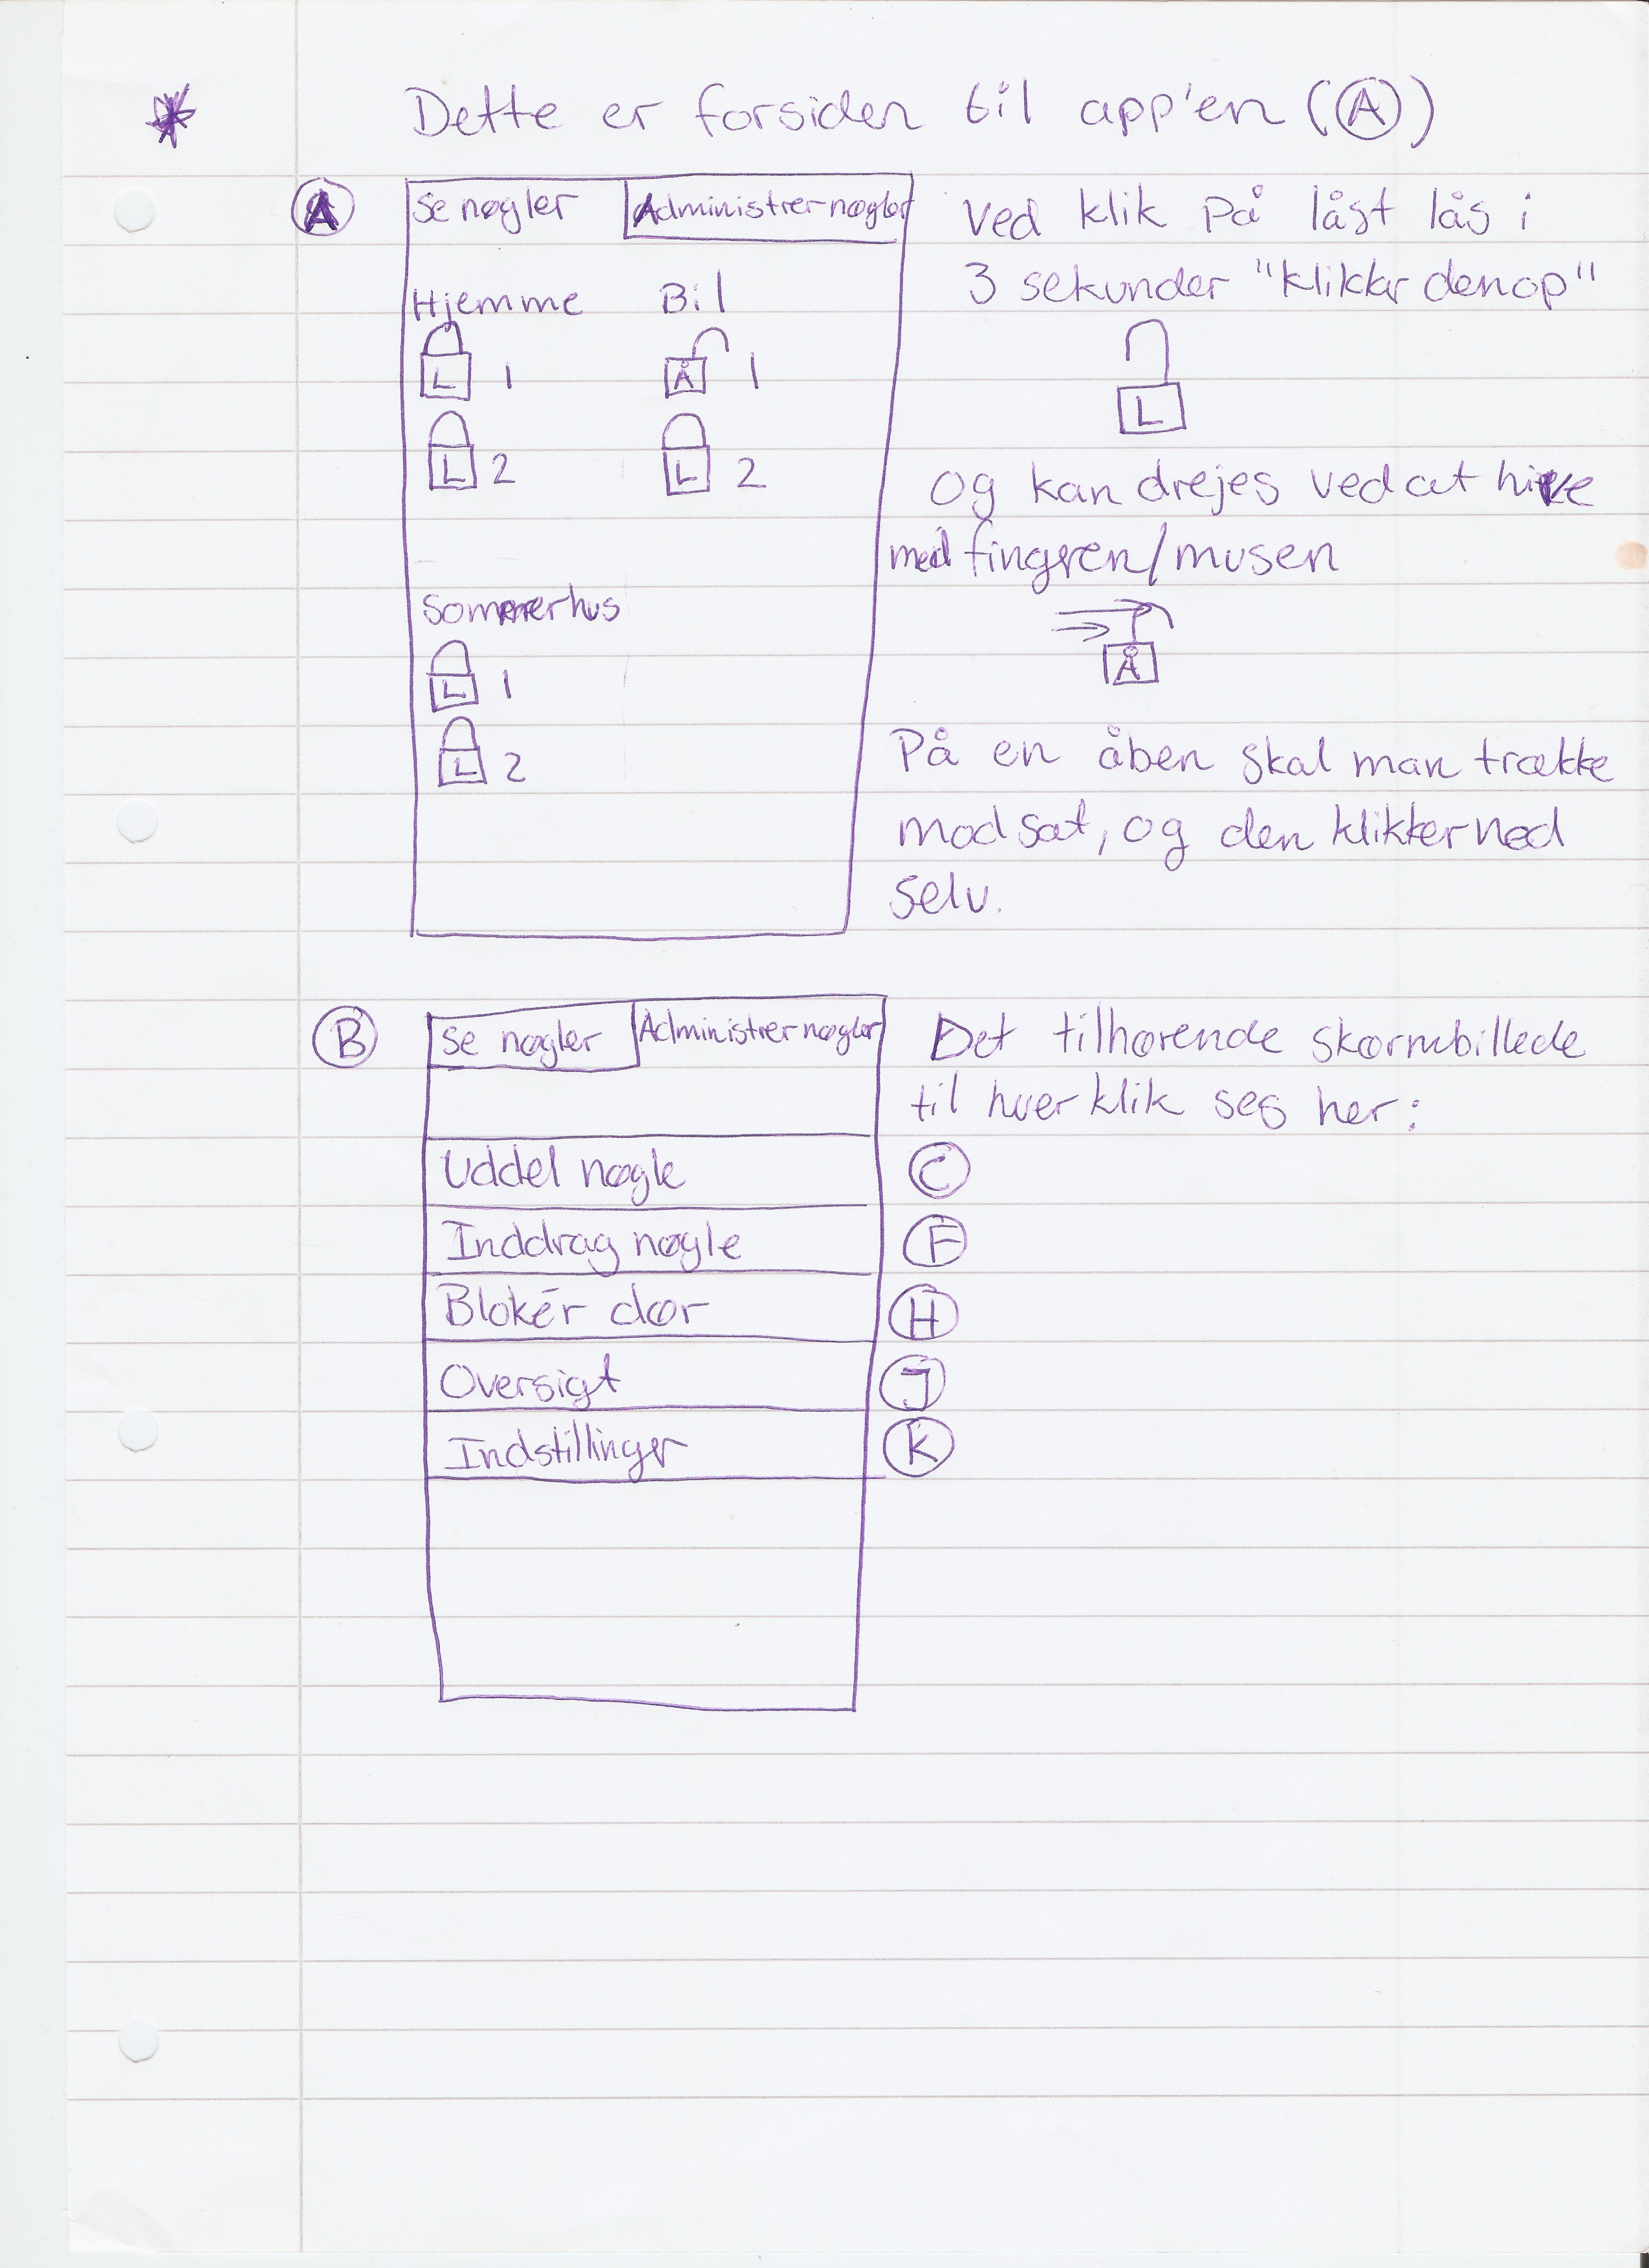
\includegraphics[width=\textwidth]{proto/AB.jpg}
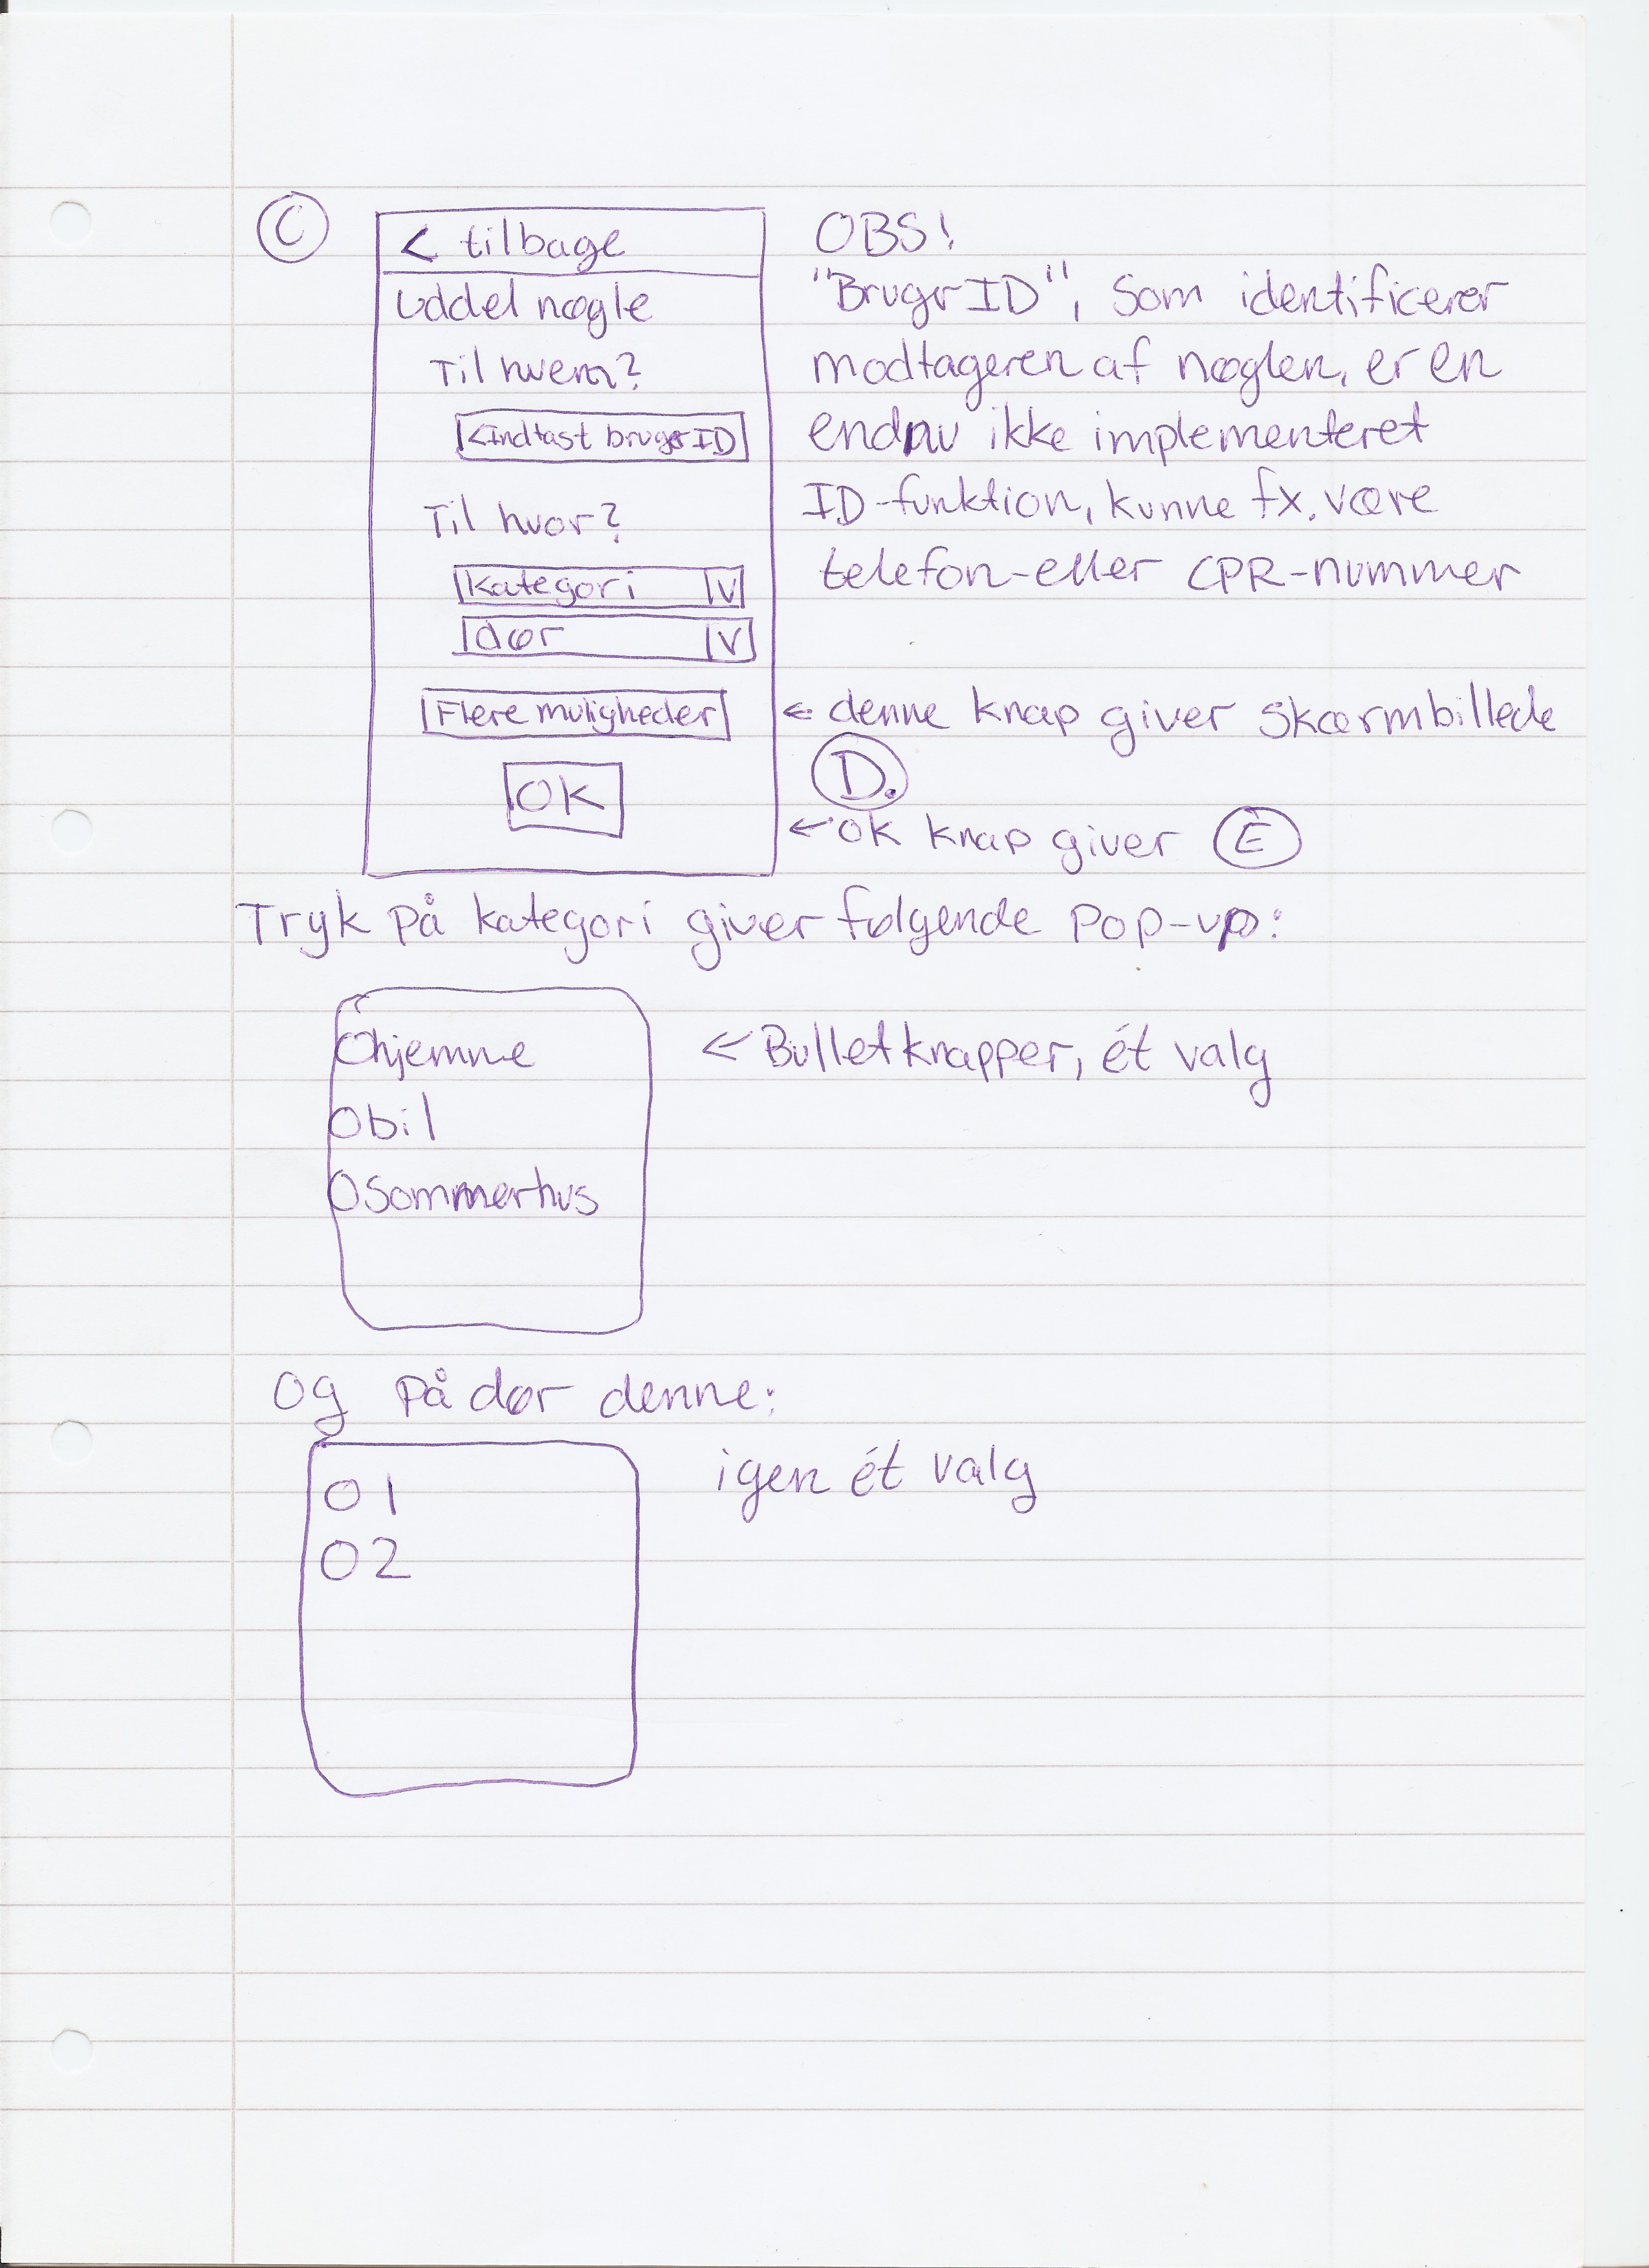
\includegraphics[width=\textwidth]{proto/C.jpg}
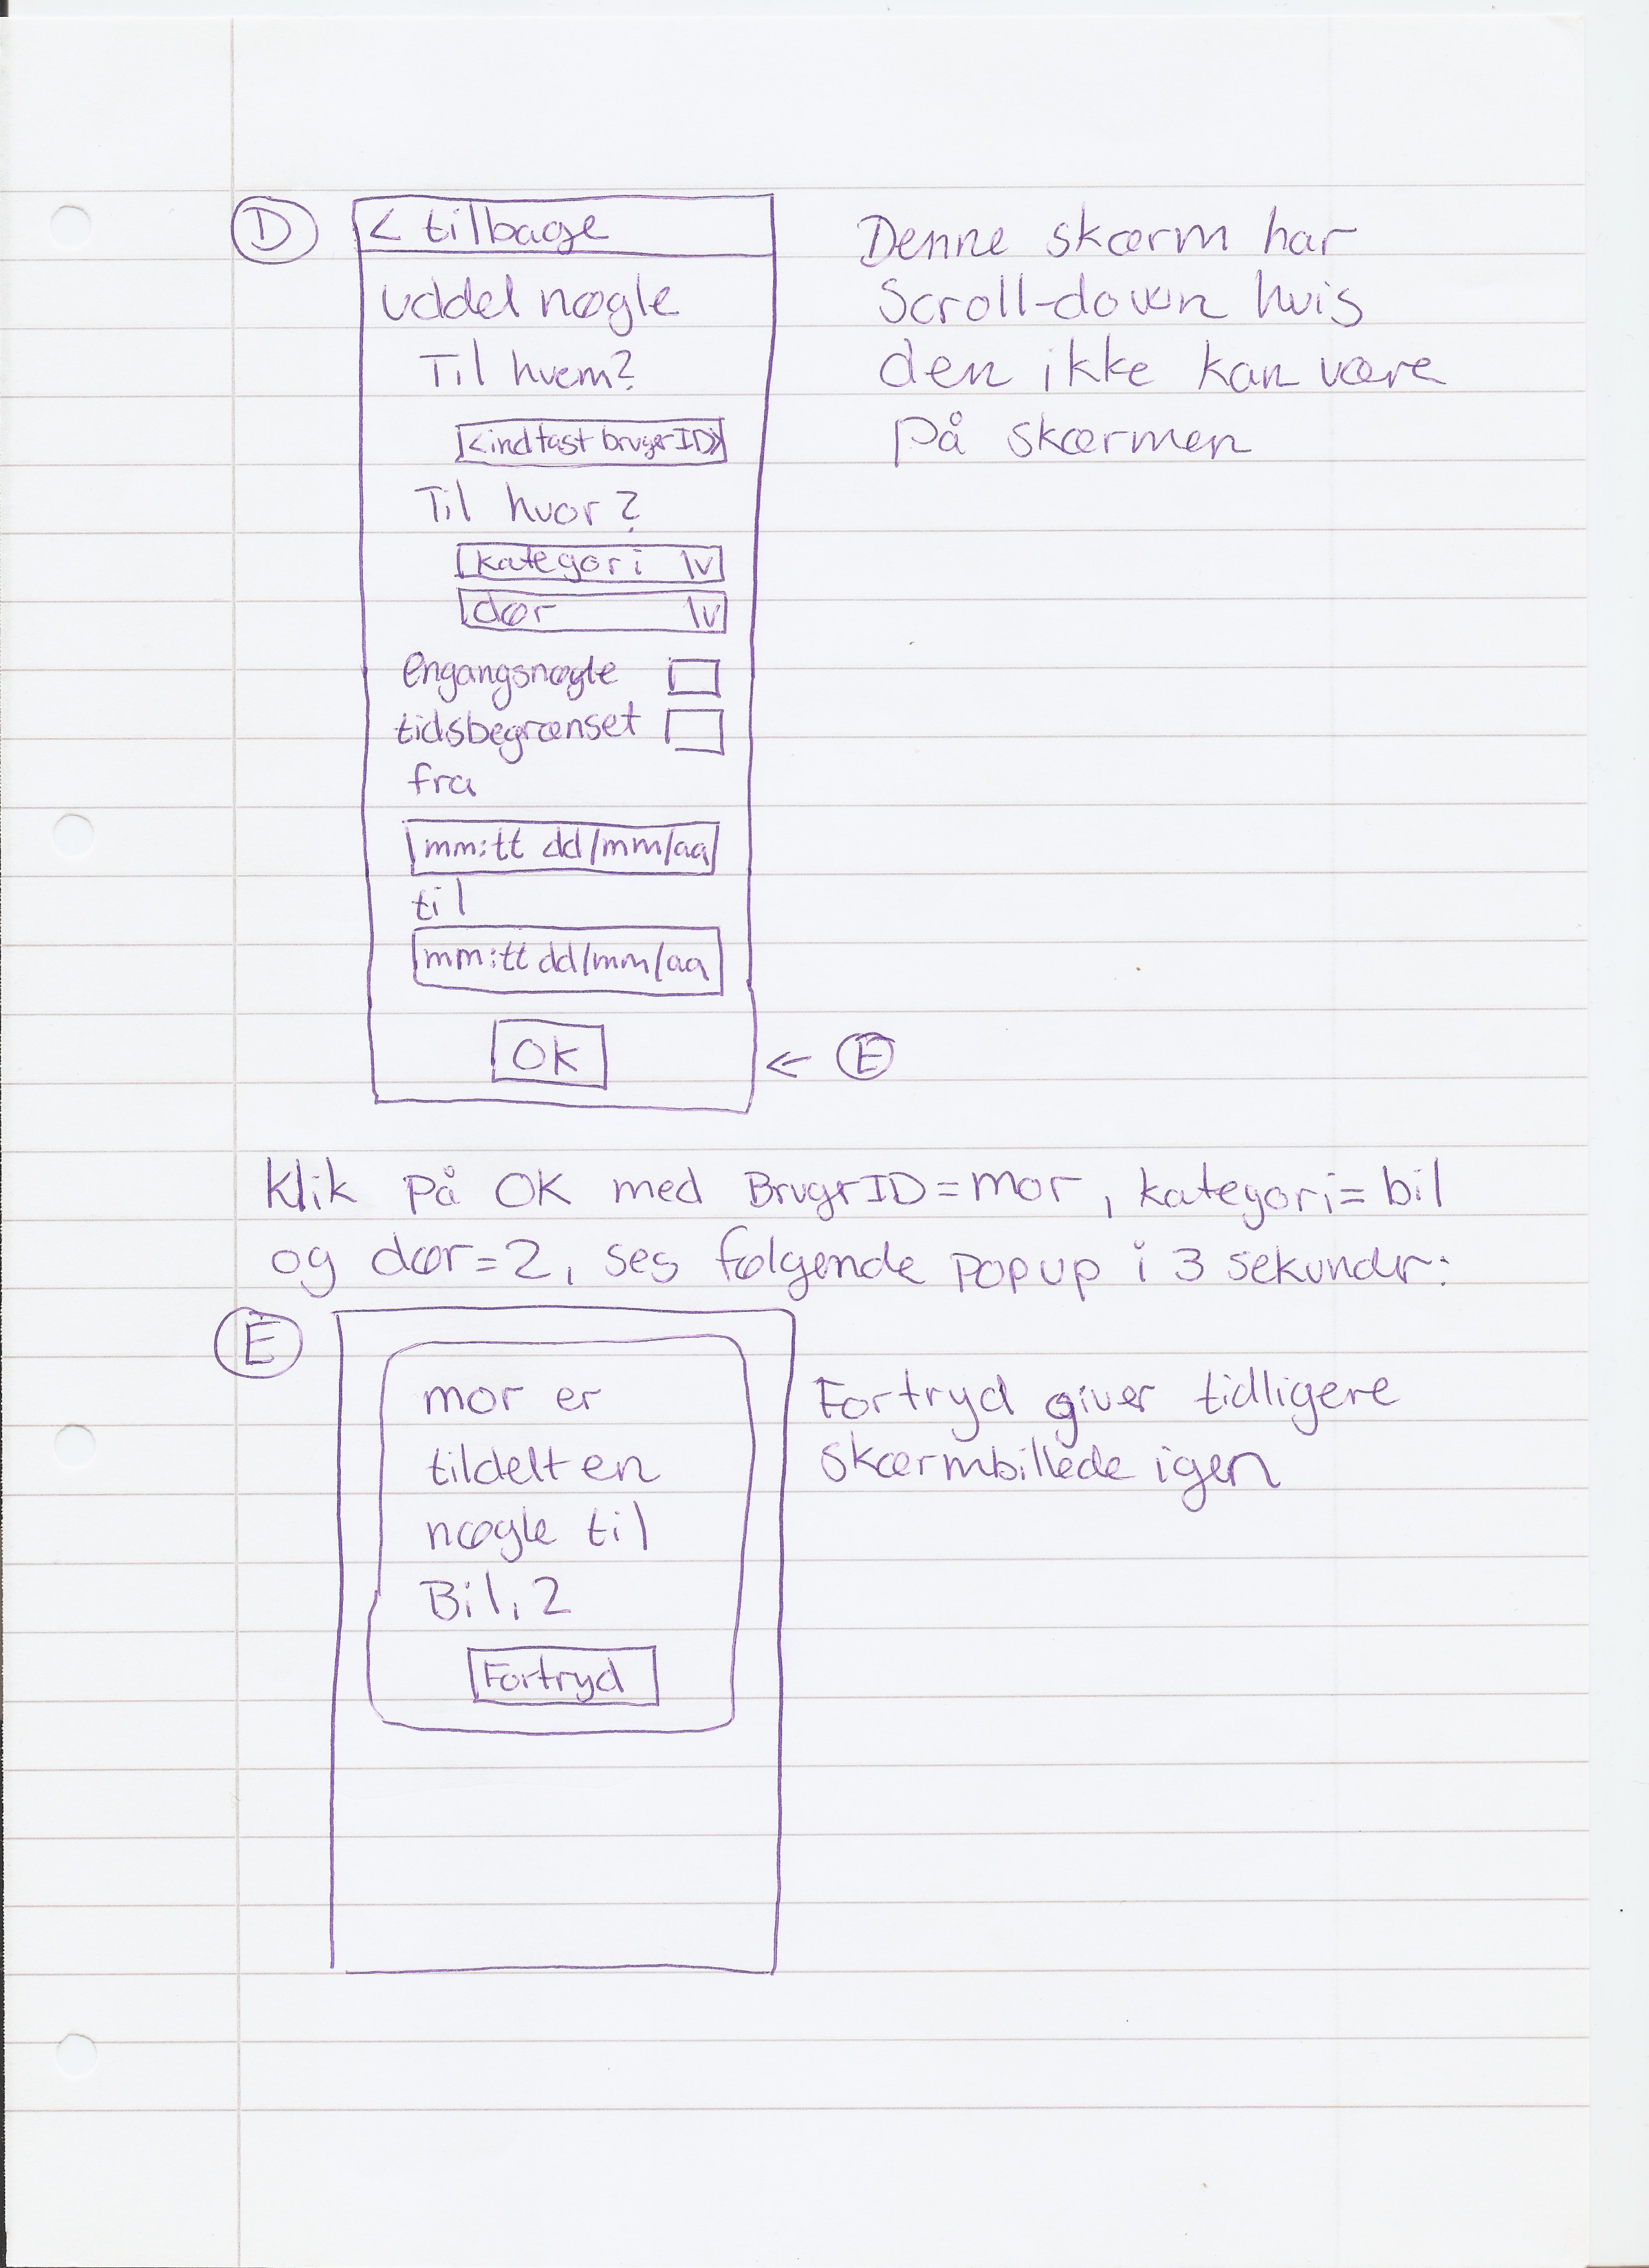
\includegraphics[width=\textwidth]{proto/DE.jpg}
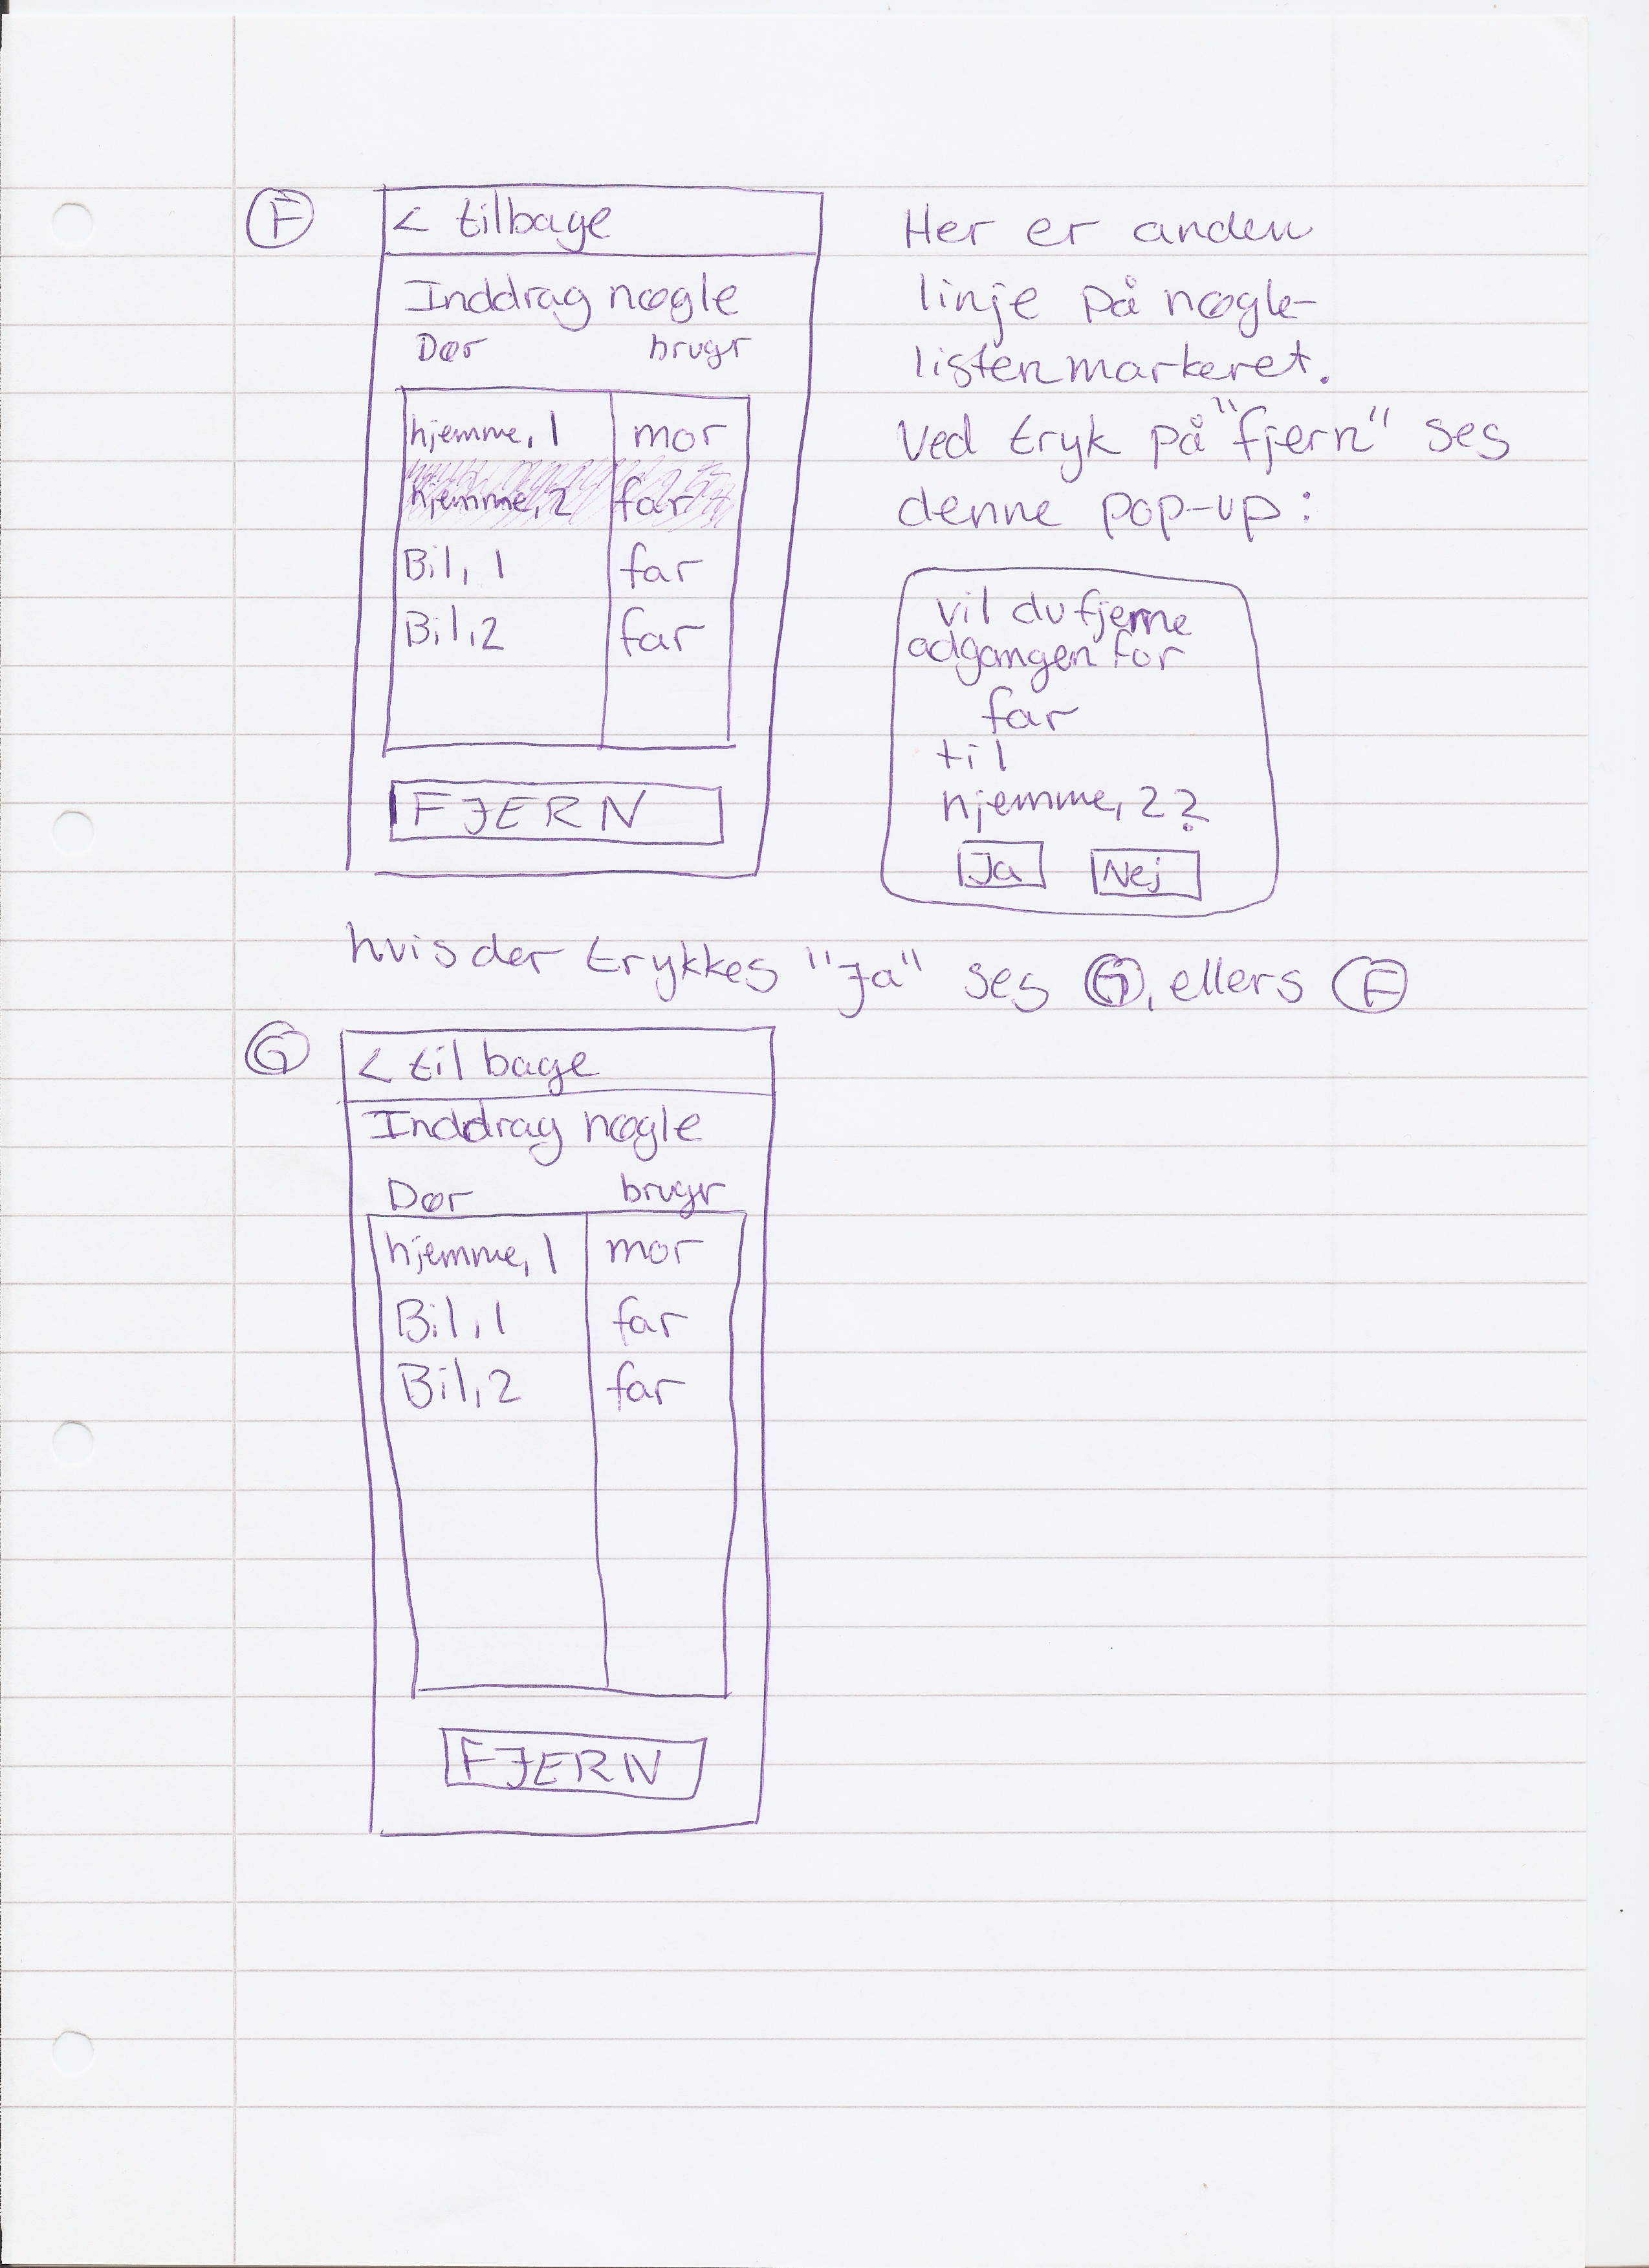
\includegraphics[width=\textwidth]{proto/FG.jpg}
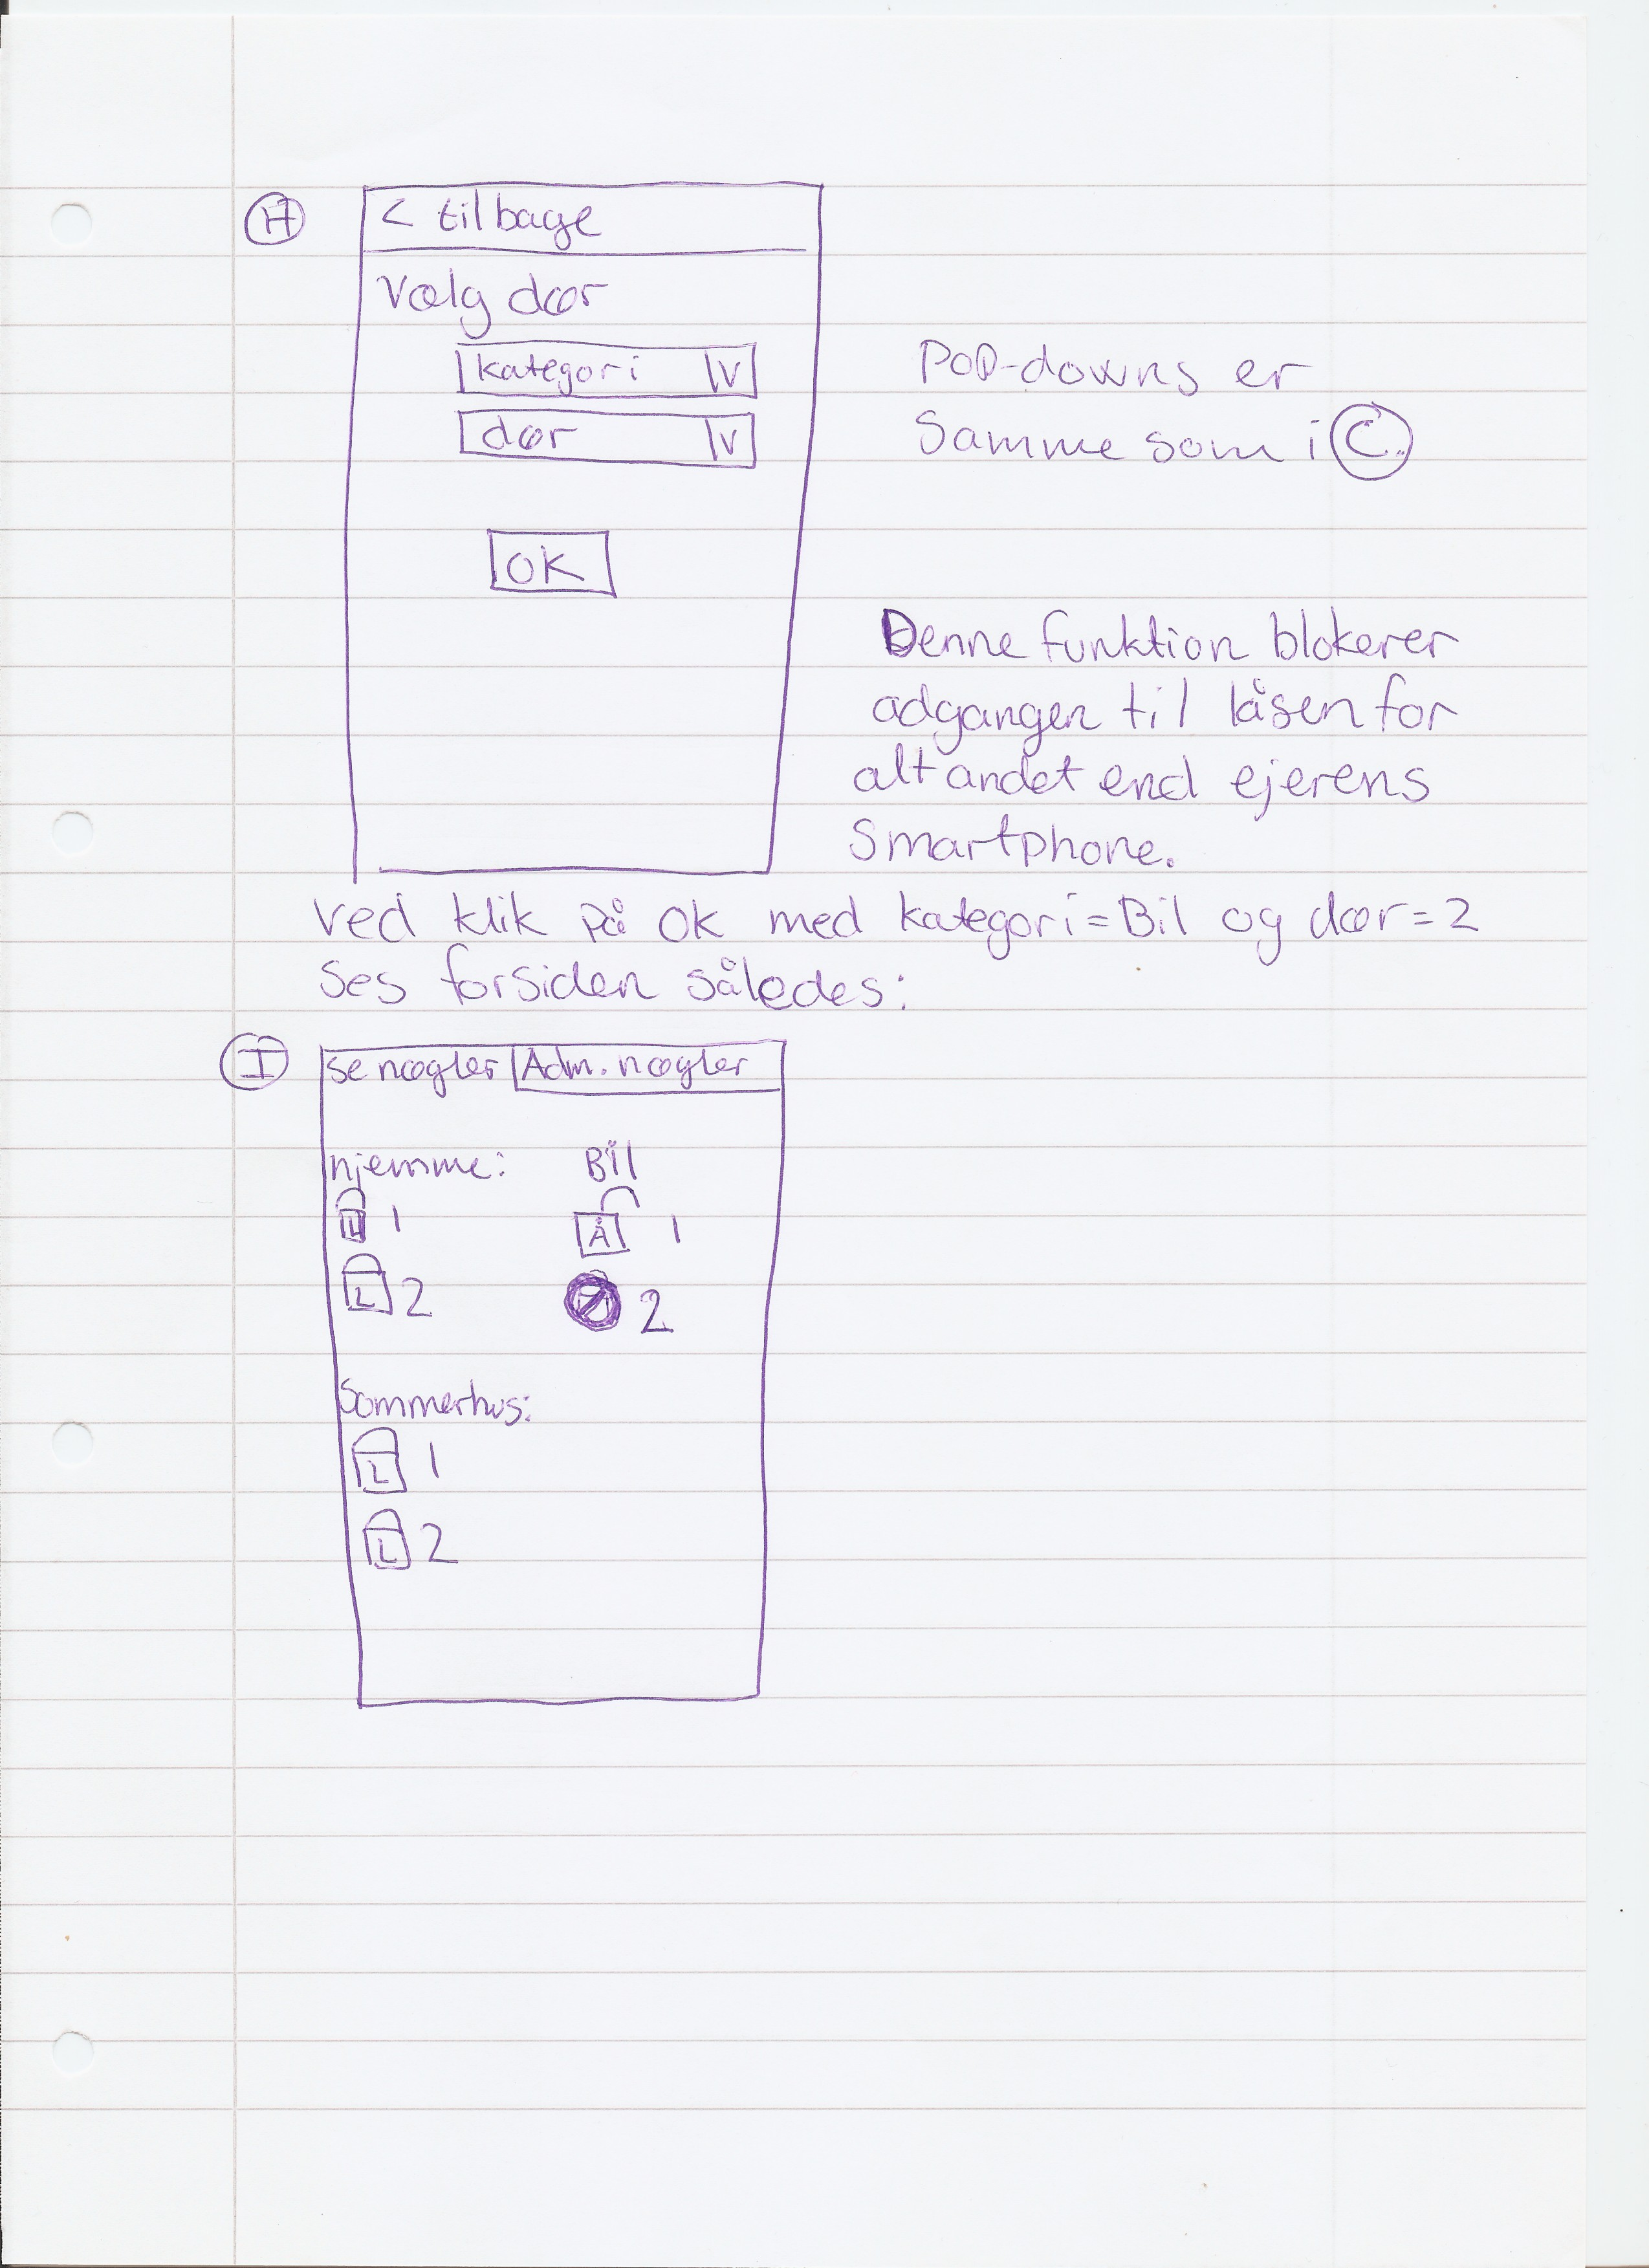
\includegraphics[width=\textwidth]{proto/HI.jpg}
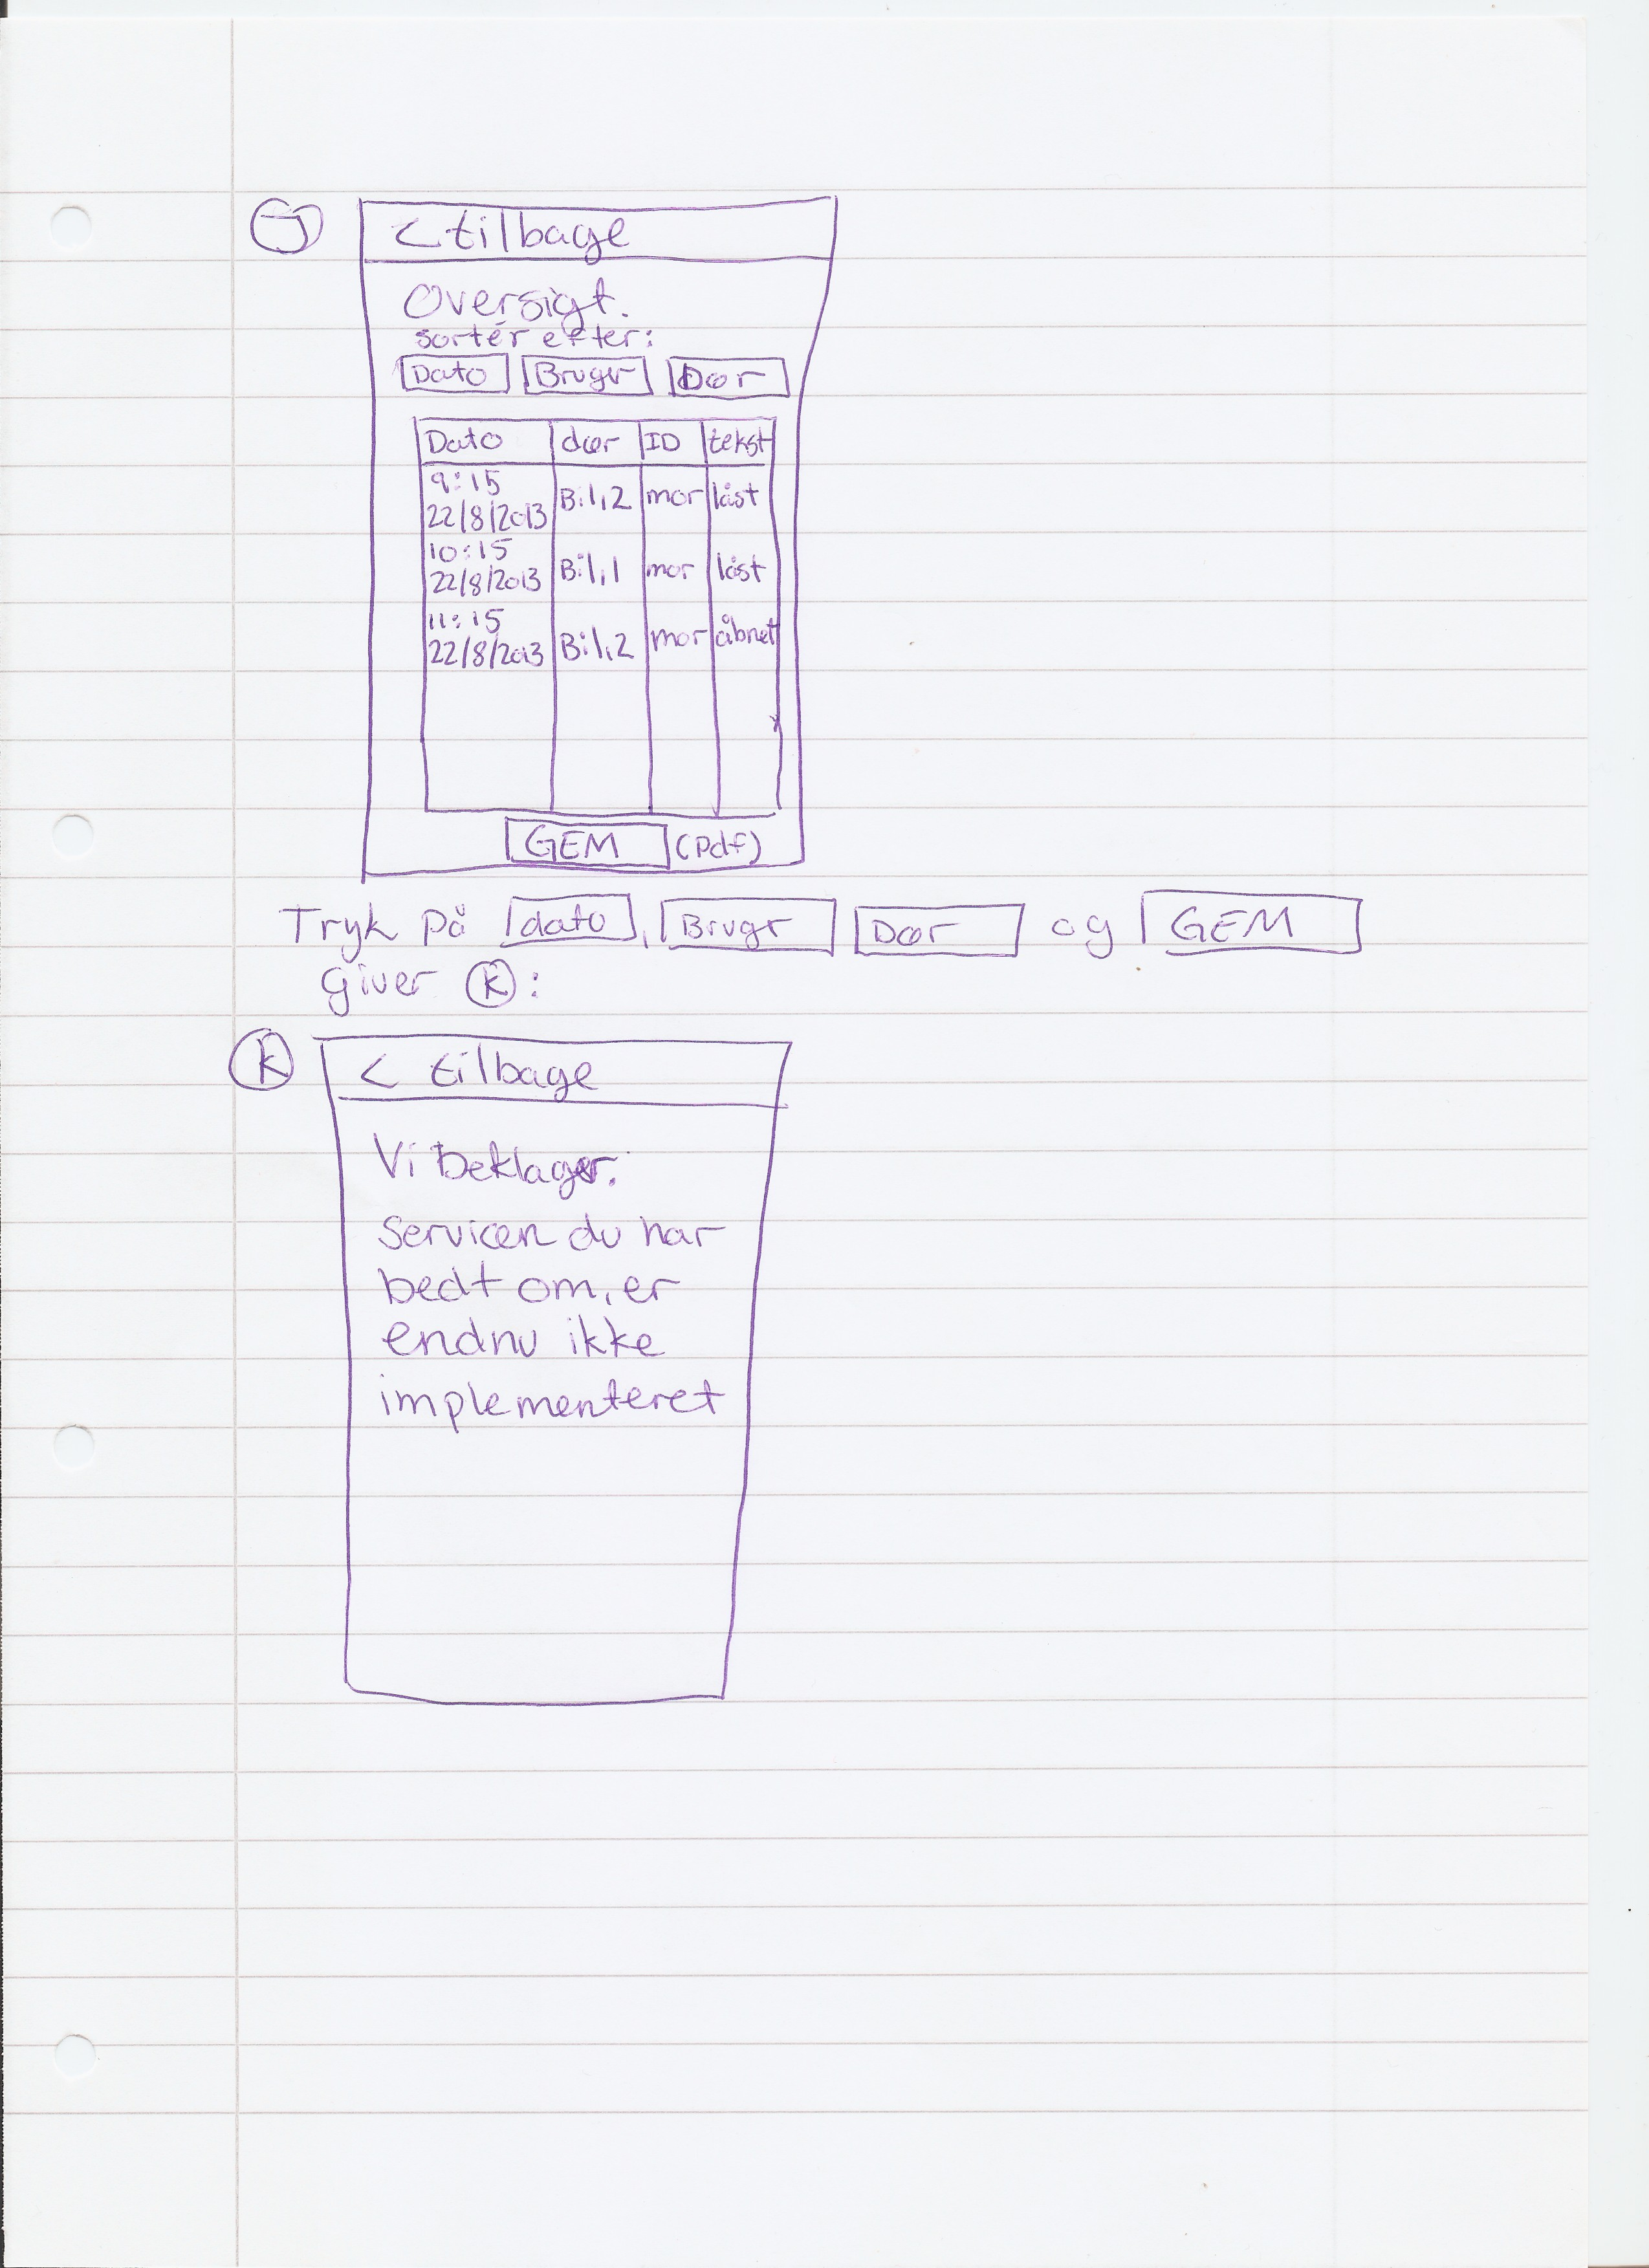
\includegraphics[width=\textwidth]{proto/JK.jpg}


\end{document}